\renewcommand*{\arraystretch}{1.1}

\subsection{Interactive / delete / 3}
\label{sec:interactive-delete-03}

% change \emph{} to use sans-serif font
\let\oldemph\emph
\renewcommand{\emph}[1]{{\footnotesize \sf #1}}

\renewcommand{\currentQueryCard}{3}
\marginpar{
  \raggedleft
  \vspace{0.22ex}

  \queryRefCard{interactive-delete-01}{ID}{1}\\
  \queryRefCard{interactive-delete-02}{ID}{2}\\ 
  \queryRefCard{interactive-delete-03}{ID}{3}\\
  \queryRefCard{interactive-delete-04}{ID}{4}\\
  \queryRefCard{interactive-delete-05}{ID}{5}\\
  \queryRefCard{interactive-delete-06}{ID}{6}\\
  \queryRefCard{interactive-delete-07}{ID}{7}\\
  \queryRefCard{interactive-delete-08}{ID}{8}\\
}


\noindent\begin{tabularx}{\queryCardWidth}{|>{\queryPropertyCell}p{\queryPropertyCellWidth}|X|}
  \hline
  query & Interactive / delete / 3 \\ \hline
  % 
  title & Remove comment like \\ \hline
  % 
  % pattern & \centering 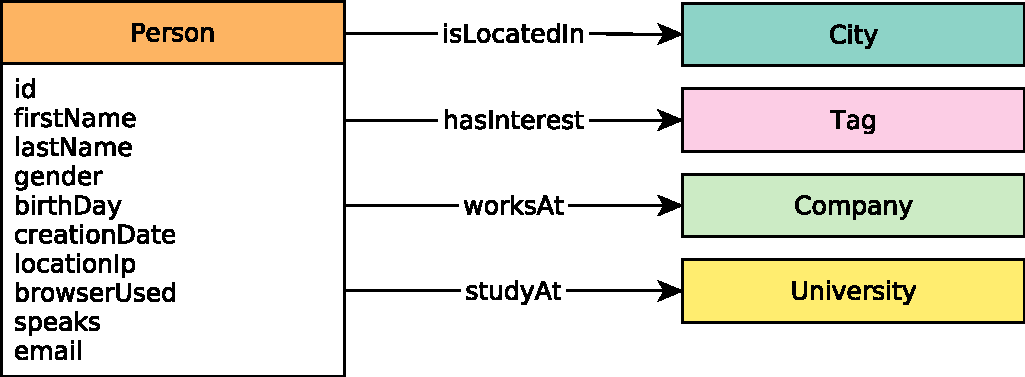
\includegraphics[scale=\patternscale,margin=0cm .2cm]{patterns/interactive-update-01} \tabularnewline \hline
  % 
  desc. & Given a \emph{Person} \textbf{node} and a \emph{Comment} \textbf{node}, remove a \emph{likes} edge between them.
  \\ \hline
  % 
  params &
  \innerCardVSpace{\begin{tabularx}{\attributeCardWidth}{|>{\paramNumberCell}c|>{\varNameCell}M|>{\typeCell}m{\typeWidth}|Y|} \hline
      $\mathsf{1}$ & Person.id
      & ID
      & \texttt{personId}
      \\ \hline
      $\mathsf{2}$ & Comment.id
      & ID
      & \texttt{commentId}
      \\ \hline
    \end{tabularx}}\innerCardVSpace \\ \hline
  % 
  comments &
  \begin{itemize}
  \item Removal a likes edge is a rare event e.g. people accidently liking a comment, this can be reflected by the relative frequency of the operation.   
  \end{itemize} 
  \\ \hline
  % 
  % 
  % 
  % 
  % 
\end{tabularx}
\queryCardVSpace

% change \emph back to the old one
\let\emph\oldemph
